
\documentclass{beamer}
\usepackage[english,brazil]{babel}
\usepackage[utf8]{inputenc}
\usepackage{graphicx}
\usepackage{minted}
\usepackage{listings}
\usepackage[T1]{fontenc}
\usetheme{Madrid}


\title{Laboratório de Segurança Cibernética}

\subtitle{"Advanced Penetration Testing, Exploits and Ethical Hacking"}

\author{Grupo do LabPentest}


\date{UFSCar, 2016}

\subject{Theoretical Computer Science}

\AtBeginSubsection[]
{
  \begin{frame}<beamer>{Agenda}
    \tableofcontents[currentsection,currentsubsection]
  \end{frame}
}

% Let's get started
\begin{document}

\begin{frame}
  \titlepage
\end{frame}

\begin{frame}{Agenda}
  \tableofcontents
  % You might wish to add the option [pausesections]
\end{frame}

% Section and subsections will appear in the presentation overview
% and table of contents.
\section{Advanced PenTesting Essentials}

\section{Network Attacks for Penetration Testers}

\section{Attacking the Domain}

\section{Exploit Linux for PenTesters}

\subsection{Introdução a Memória}

\begin{frame}{Memória Física}

  \begin{itemize}
  \item{
  Registradores
  \begin{itemize}
    \item{
    Propósito Geral (EAX, EBX, ECX, EDX, ESI, EDI, EBP, ESP), Segmento (CS, DS, SS, ES, FS, GS), Eflags, EIP.
    }
  \end{itemize}
  }
  \begin{figure}[tbp]
        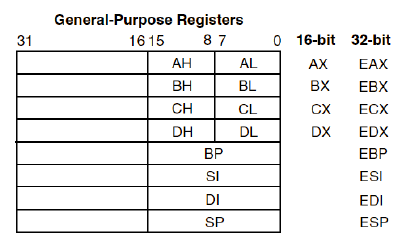
\includegraphics[width=5cm, height=3cm]{Linux/imagens/general_purpose_registers.png}
        \break
        \centering
    \end{figure}
  \item{
  Cache
  }
  \item{
  RAM
  }
\end{itemize}
\end{frame}

\begin{frame}{Memória}
  \begin{itemize}
  \item{
  Modos de Endereçamento
  \begin{itemize}
    \item{
        Modo Real
    }
    \item{
        Modo Protegido
    }
  \end{itemize}
  }
  \item{
  Memória Virtual
  \begin{itemize}
    \item{
        Memória Física
    }
    \item{
        Endereçamento Linear
    }
  \end{itemize}
  }
  \item{
  Paginação
  }
\end{itemize}
\end{frame}

\begin{frame}{Paginação}
  \begin{itemize}
  \item{
  Permite endereçamento indireto da memória
  }
  \item{
  O endereçamento linear é mapeado em páginas de tamanho fixo
  \begin{itemize}
    \item{
        Normalmente de tamanho 4KB
    }
    \item{
        Páginas são indexadas por tabelas de páginas com 1.024 entradas
    }
    \item{
        Tabelas de Páginas são mapeadas em Diretórios de Páginas
    }
    \item{
        Tradução do endereço virtual para o endereço real
    }
    \item{
        TLB
    }
  \end{itemize}
  }
  \item{
  Troca de Contexto
  }
  \item{
  Páginas que não foram acessadas recentemente são copiadas de volta ao disco
  }
  \item{
  Page Fault
  }
\end{itemize}
\end{frame}

\begin{frame}{Arquivo Objeto}
  \begin{itemize}
  \item{
  Segmento de Código
  }
  \item{
  Segmento de Dados
  }
  \item{
  Segmento BSS
  }
  \item{
  Heap
  }
  \item{
  Pilha
  }
\end{itemize}
\end{frame}

\begin{frame}[fragile]
  \frametitle{Demonstração dos Segmentos}
  \begin{columns}
    \begin{column}{0.5\textwidth}
    \end{column}
    \begin{column}{0.5\textwidth}
      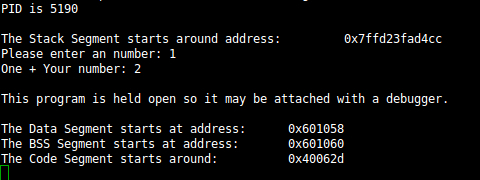
\includegraphics[width=.99\linewidth]{Linux/imagens/LabPentest1.png}
    \end{column}
  \end{columns}
\end{frame}

\begin{frame}[fragile]
  \frametitle{Pilha}
  \begin{columns}
    \begin{column}{0.5\textwidth}
    \begin{itemize}
        \item{
          Funções
        }
         \item{
        LIFO
        }
        \item{
          Ponteiro de Retorno
          }
         \item{
          Buffer
          } 
          \item{
          Procedure Prolog
          \begin{itemize}
            \item{
                push \%ebp
            }
            \item{
                mov \%esp,\%ebp
            }
            \item{
                sub 0x8,\%esp
            }
          \end{itemize}
          } 
          \item{
          Procedure Epilog
          \begin{itemize}
            \item{
                mov \%ebp,\%esp
            }
            \item{
                pop \%ebp
            }
            \item{
                ret
            }
          \end{itemize}
          } 
        \end{itemize}
    \end{column}
    \begin{column}{0.5\textwidth}
      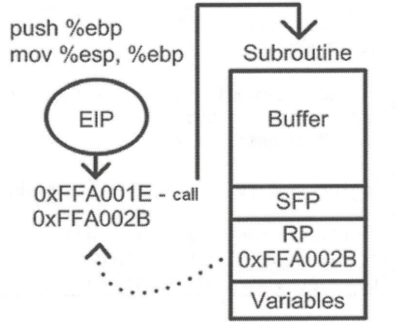
\includegraphics[width=.99\linewidth]{Linux/imagens/LabPentest2.png}
    \end{column}
  \end{columns}
\end{frame}


\begin{frame}{Ferramenta: GNU Debugger (GDB)}
  \begin{itemize}
  \item{
  Debugger para as linguagens C, C++ e Fortran
  }
  \item{
  Alguns Comandos:
    \begin{itemize}
        \item{
             disass "function" - Mostra as instruções assembly de uma função
        }
        \item{
             break "function" - Pausa a execução quando a função especificada é alcançada
        }
        \item{
             print - Imprime conteúdo de registradores e variáveis
        }
        \item{
             x/"number"i "mem address" - Examina localizações na memória
        }
        \item{
             info - Imprime o conteúdo e o estado de registradores e variáveis
        }
    \end{itemize}
  }
\end{itemize}
\end{frame}

\begin{frame}[fragile]
  \frametitle{Demonstração da Ferramenta GBD}
      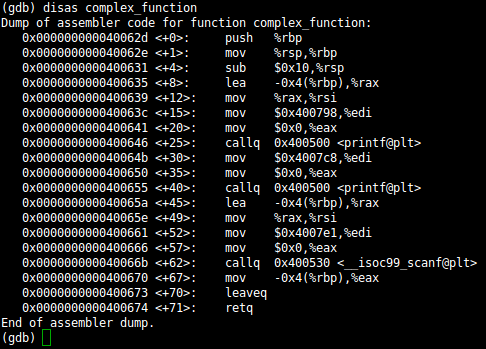
\includegraphics[width=.99\linewidth]{Linux/imagens/LabPentest3.png}
\end{frame}

\begin{frame}[fragile]
  \frametitle{Linguagem Assembly x86}
  \begin{itemize}
      \item {
        Linguagem de baixo nível
      }
  \end{itemize}
  \begin{columns}
    \begin{column}{0.5\textwidth}
        \begin{itemize}
            \item {
                AT\&T
              }
            \item{
              pushI \$8 \linebreak
              mov \%esp,\%ebp
            }  
            \item{
              Primeiro src, depois dest
            }  
            \item{
            \$ = Operando Imediato
            }
            \item{
            \% = Operando Indireto
            }
            \item{
            () = Ponteiro
            }
            \item{
            Tamanho dos Operandos
                \begin{itemize}
                    \item {
                      movI \$0x8028024,(\%esp)
                    }
                    \item{
                     b - byte, w - word, l - long
                    }
                \end{itemize}
            }
        \end{itemize}
    \end{column}
    \begin{column}{0.5\textwidth}
        \begin{itemize}
            \item {
                Intel
              }
            \item{
              push 8 \linebreak
              mov ebp, esp
            }  
            \item{
              Primeiro dest, depois src
            }  
            \item{
            [] = Ponteiro
            }
            \item{
            Tamanho dos Operandos
                \begin{itemize}
                    \item {
                      mov DWORD PTR [esp],0x8028024
                    }
                    \item{
                     Intel usa “byte ptr”, “word ptr”, ou “dword ptr”
                    }
                \end{itemize}
            }
        \end{itemize}
    \end{column}
  \end{columns}
\end{frame}

\begin{frame}{Linkers \& Loaders}
    \begin{itemize}
        \item {
        Linkers: ligam o nome de uma função para sua localização real
        }
        \item{
        Loaders: Carregam um programa da unidade de armazenamento (disco) para a memória
        }
        \item{
        Resolução de Símbolos: resolução do endereço das funções em tempo de execução
        }
        \item{
        Relocação: conflitos de endereçamento requerem relocação
        }
        \item{
        "Name Mangling": A função main se torna \_main ou Z\_main\_\
        }
    \end{itemize}
  
\end{frame}

\begin{frame}{ELF - Executable and Linking Format}
  \begin{itemize}
      \item {
      Arquivos Relocáveis
      }
      \item{
      Arquivos Executáveis
      }
      \item{
      Objetos Compartilhados
      }
      \item{
      Global Offset Table (GOT)
      }
      \item{
      Procedure Linkage Table (PLT)
      }
  \end{itemize}
\end{frame}

\begin{frame}{Ferramenta: objdump}
  \begin{itemize}
      \item {
      Exibe informações do arquivo objeto
      }
      \item{
      Realiza disassembly, assim como GDB, mas com objdump não é necessário executar o arquivo
      }
      \item{
      Comandos:
        \begin{itemize}
            \item {
                objdump -d: Realiza o disassembly de um arquivo objeto
            }
            \item{
                objdump -j "section name": Permite especificar uma seção
            }
            \item{
                objdump -h: Exibe os headers das seções
            }
        \end{itemize}
      }
  \end{itemize}
\end{frame}

\begin{frame}{Ferramenta: readelf}
  \begin{itemize}
      \item{
      Exibe informações dos headers do arquivo objeto ELF e das seções: GOT, PLT, e informações de localização
      }
  \end{itemize}
\end{frame}

\begin{frame}{Demonstração das Ferramentas}
 
    GBD: disas main \linebreak
        
\includegraphics[width=.8\linewidth]{Linux/imagens/LabPentest4.png} \linebreak
    objdump -d -j .text memtest | grep puts \linebreak
     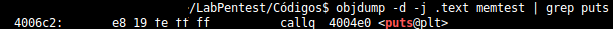
\includegraphics[width=.8\linewidth]{Linux/imagens/LabPentest5.png} \linebreak
    objdump -R memtest \linebreak
    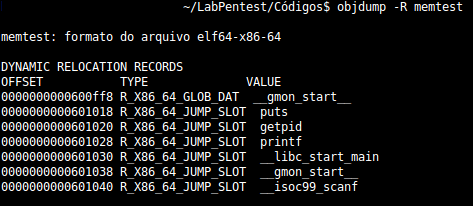
\includegraphics[width=.8\linewidth]{Linux/imagens/LabPentest6.png} \linebreak

\end{frame}

\begin{frame}{Demonstração das Ferramentas}
 
    Analisando a função puts() - disas put: \linebreak
        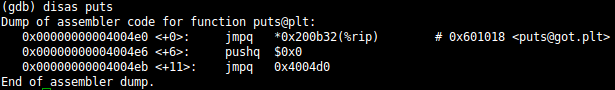
\includegraphics[width=.8\linewidth]{Linux/imagens/LabPentest7.png} \linebreak
    readelf -x 22 memtest \linebreak
     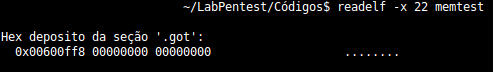
\includegraphics[width=.8\linewidth]{Linux/imagens/LabPentest8.png} \linebreak
    Depois de executar o programa memtest e determinar o endereço da GOT:
    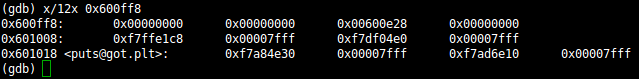
\includegraphics[width=.8\linewidth]{Linux/imagens/LabPentest9.png}
    

\end{frame}

\begin{frame}{Heap}
    \begin{columns}
    \begin{column}{0.6\textwidth}
    \begin{itemize}
        \item{
          Memória Dinâmica alocada em tempo de execução
        }
        \item{
            A memória é liberada por:
            \begin{itemize}
                \item {
                Código, Garbage Colector ou pelo fim do programa
                }
            \end{itemize}
        }
        \item{
        Segmento de Código armazena instruções executáveis
        }
        \item{
        Segmento de Dados armazena variáveis globais e estáticas
        }
        \item{
        BSS armazena código não inicializdo
        }
        \item{
        Heap é usada para todas as outras variáveis do programa
        }
    \end{itemize}
    \end{column}
    \begin{column}{0.4\textwidth}
      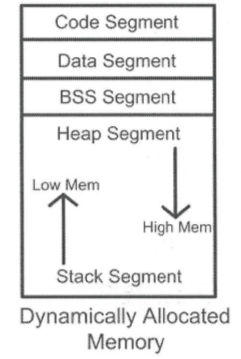
\includegraphics[width=.8\linewidth]{Linux/imagens/heap.png}
    \end{column}
  \end{columns}
  
\end{frame}

\begin{frame}{Memória Dinâmica}
    \begin{itemize}
        \item {
            malloc
            \begin{itemize}
                \item {
                Interface para chamadas de sistema sbrk() e mmap()
                }
                \item{
                Quebra a alocação de memória do sbrk() e do mmap() em chunks menores
                }
                \item{
                malloc(), realloc(), free()
                }
            \end{itemize}
        }
        \item{
            dlmalloc: Implementação do Malloc por Doug Lea
        }    
    \end{itemize}
\end{frame}

\begin{frame}[fragile]
  \frametitle{Memória Dinâmica}
  \begin{columns}
    \begin{column}{0.5\textwidth}
      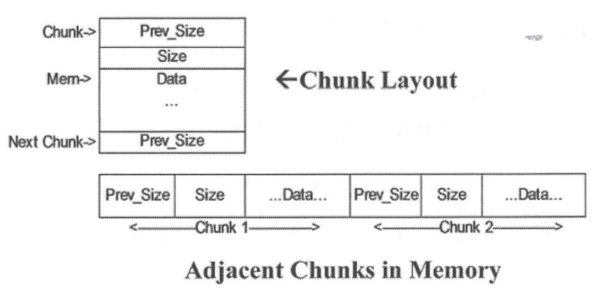
\includegraphics[width=.99\linewidth]{Linux/imagens/ChunkLayout.png}
    \end{column}
    \begin{column}{0.5\textwidth}
      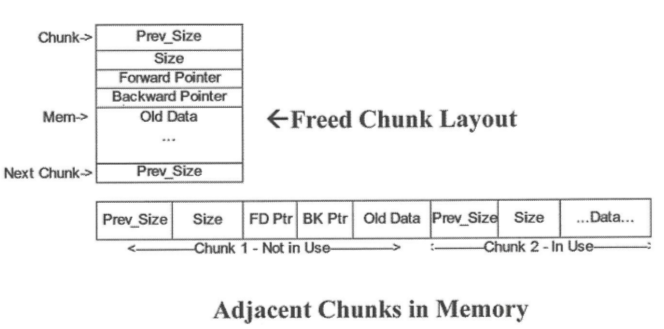
\includegraphics[width=.99\linewidth]{Linux/imagens/FreedChunkLayout.png}
    \end{column}
  \end{columns}
\end{frame}

\begin{frame}{Memória Dinâmica}
    \begin{itemize}
        \item {
            Funções unlink() e frontlink():
            \begin{itemize}
                \item {
                unlink(): remove chunks de uma lista duplamente ligada. Chamada por free() quando um chunk adjacente está inutilizado.
                }
                \item{
                frontlink(): insere novos chunks em uma lista duplamente ligada
                }
            \end{itemize}
        }
    \end{itemize}
\end{frame}

\begin{frame}[fragile]
  \frametitle{Unlink e o Processo de Fusão}
  \begin{columns}
    \begin{column}{0.5\textwidth}
      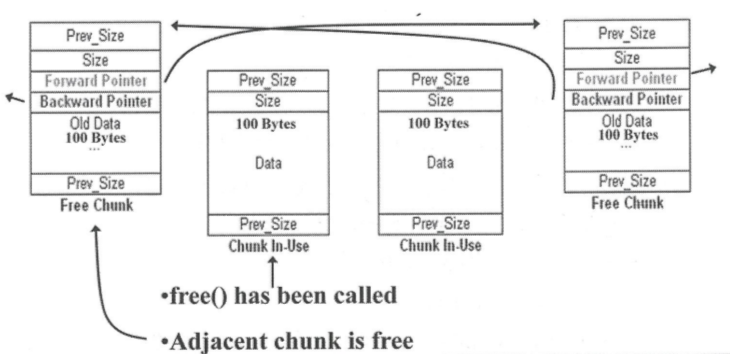
\includegraphics[width=.99\linewidth]{Linux/imagens/Unlink1.png}
    \end{column}
    \begin{column}{0.5\textwidth}
      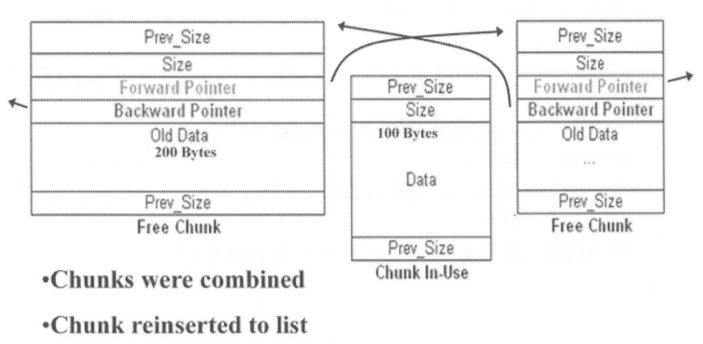
\includegraphics[width=.99\linewidth]{Linux/imagens/Unlink2.png}
    \end{column}
  \end{columns}
\end{frame}

\begin{frame}{Ferramenta: Itrace}
    \begin{itemize}
        \item {
            Ferramenta para interceptar e gravar chamadas a bibliotecas. É util para localizar chamadas para alocação de memória.
        }
        \item{
            Similar a ferramenta strace
        }
        \item{
            Pode ser utilizada para encontrar o endereço de memória do chunk alocado pelo malloc:
        }
    \end{itemize}
    
\end{frame}

\begin{frame}{ShellCode}
    \begin{itemize}
        \item {
            Tem esse nome porque foi primariamente utilizado para lançar um shell.
        }
        \item{
            Escrito em linguagem Assembly, específico de cada tipo de processador. É convertido para linguagem de máquina por um assembler, como o NASM.
        }
        \item{
            Injetado em um programa, serve como payload.
        }
        \item{
            Quando convertido para código de máquina, os bytes nulos devem ser eliminados. Funções como strcpy() terminam quando encontram algum byte nulo
        }
        \item{
            Ferramenta NASM: Usada para montar código assembly em arquivos objeto.
        }
    \end{itemize}
    
\end{frame}

\begin{frame}{Chamadas de Sistema}
    \begin{itemize}
        \item {
            Maneira de comunicação entre o user mode e o kernel mode
        }
        \item{
            Argumentos são carregados na memória e uma interrupção é feita
            \begin{itemize}
                \item {
                EAX armazena o número da chamada de sistema
                }
                \item{
                EBX, ECX e EDX normalmente armazenam os argumentos
                }
            \end{itemize}
        }
    \end{itemize}
    
\end{frame}

\begin{frame}{Criando ShellCode}

    ShellCode para restaurar direitos de root (usando syscall setruid()):
  colocar aqui codigo shellcode\_w\_zeros
\end{frame}

\begin{frame}{Criando ShellCode}
    \begin{itemize}
        \item {
        Utilizando a ferramenta NASM para criar o shellcode. O comando xxd -ps exibe o codigo de máquina em hexadecimal:
        }
    \end{itemize}
    \begin{center}
     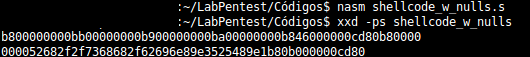
\includegraphics[width=.8\linewidth]{Linux/imagens/LabPentest10.png}
    \end{center} 
     \begin{itemize}
         \item {
         Existem muitos bytes nulos. Funções de manipulação de strings vão falhar.
         }
         \item{
         É necessário remover os bytes nulos.
         \begin{itemize}
             \item {
             mov eax, 0x00 ;Esse comando deixa 0's sobrando
             }
             \item{
             mov al, 0x00 ;Melhor maneira de evitar bytes nulos
             }
         \end{itemize}
         }
         \item{
         ShellCode com os bytes nulos removidos:
         }
     \end{itemize}
     \begin{center}
     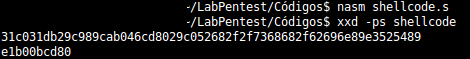
\includegraphics[width=.8\linewidth]{Linux/imagens/LabPentest11.png}
     \end{center}

\end{frame}


\subsection{Exemplos de Ataques ao Domínio Linux}

\begin{frame}{Runtime Attacks}
    \begin{itemize}
        \item {
            Controle da aplicação é comprometido em tempo de execução
        }
        \item{
            Tipicamente, ocorre a injeção de código malicioso
        }
        \item{
            Esses tipos de ataques são possíveis pelo fato de o software ser escrito deixando vulnerabilidades
        }
        \item{
            Exemplo mais comum de ataque: Buffer Overflow
        }
    \end{itemize}
    
\end{frame}

\begin{frame}{Contramedidas}
  \begin{itemize}
      \item{Writable Xor Executable
        \begin{itemize}
            \item {
                Previne a execução de código injetado marcando as páginas como \textit{writable} ou \textit{executable}
            }
            \item{
                Implementado no Linux [PaXa] e no Windows [DEP]
            }
            \item{
                Intel e AMD oferecem suporte
            }
        \end{itemize}
      }
      \item{
        ASLR - Address Space Layout Randomization
        \begin{itemize}
            \item {
                O endereço base dos segmentos de memória é randômico
            }
        \end{itemize}
      }
      \item{
        Extensões do compilador
        \begin{itemize}
            \item {
                Dificultam buffer oveflow adicionando canarios de pilha (stack canaries), verificadores de limites, reordenação de variáveis, etc.
            }
        \end{itemize}
      }
  \end{itemize}
\end{frame}

\begin{frame}{Buffer Overflow}
  \begin{itemize}
      \item {
        Objetivo: Mudar o fluxo de execução de um programa redirecionando para um código malicioso injetado.
      }
      \item{
        Injeção de Código:
        \begin{itemize}
            \item {
                Código pode ser injetado realizando overflow de um buffer local alocado na pilha
            }
            \item{
                Esse código é referenciado como \textcolor{red}{shellcode}
            }
            \item{
                Pode ser utilizado para dar acesso a um shell root ao atacante, estabelecer um backdoor na máquina, entre outros tipos de ataques.
            }
        \end{itemize}
      }
  \end{itemize}
\end{frame}

\defverbatim[colored]\lstI{
\begin{lstlisting}[language=C++,basicstyle=\ttfamily,keywordstyle=\color{blue}]
#include <stdio.h>
void echo()
{
    char buffer[80];
    gets(buffer);
    puts(buffer) ;
}
int main()
{
    echo();
    printf ("Done");
    return 0;
}
\end{lstlisting}
}

\begin{frame}{Buffer Overflow}
    \begin{itemize}
        \item {Código vulnerável:
        \begin{itemize}
            \item {
                A função gets() não faz checagem de fronteiras
            }
        \end{itemize}
        }
    \end{itemize}
    \lstI
\end{frame}

\begin{frame}{Buffer Overflow}
    \begin{center}
       (1) O programa começa
       \linebreak
       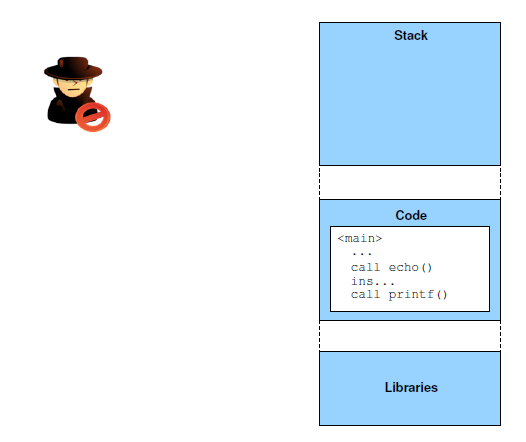
\includegraphics[width=.65\linewidth]{Linux/imagens/bo1.PNG}
    \end{center}

\end{frame}

\begin{frame}{Buffer Overflow}
    \begin{center}
       (2) A função echo() é chamada
       \linebreak
       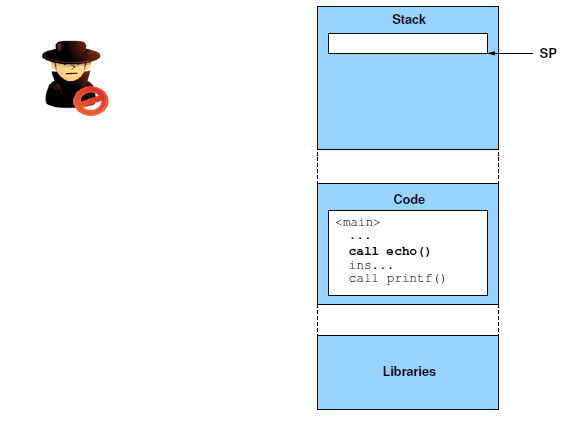
\includegraphics[width=.65\linewidth]{Linux/imagens/bo2.PNG}
    \end{center}

\end{frame}

\begin{frame}{Buffer Overflow}
    \begin{center}
       (3) A instrução call faz o push do endereço de retorno na pilha
       \linebreak
       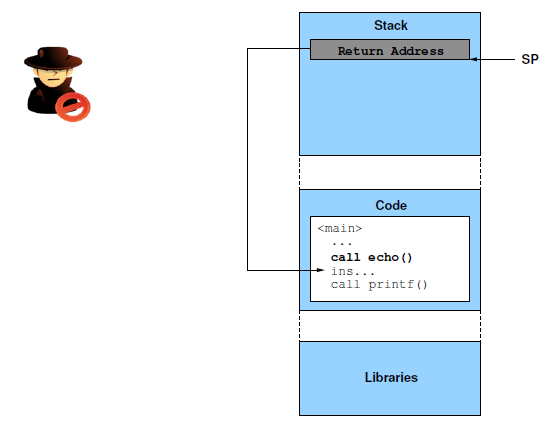
\includegraphics[width=.65\linewidth]{Linux/imagens/bo3.PNG}
    \end{center}

\end{frame}

\begin{frame}{Buffer Overflow}
    \begin{center}
       (4) Espaço do buffer é alocado na pilha
       \linebreak
       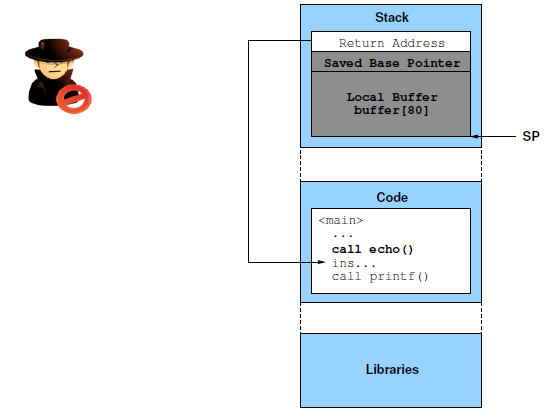
\includegraphics[width=.65\linewidth]{Linux/imagens/bo4.PNG}
    \end{center}

\end{frame}

\begin{frame}{Buffer Overflow}
    \begin{center}
       (5) echo() chama gets(buffer)
       \linebreak
       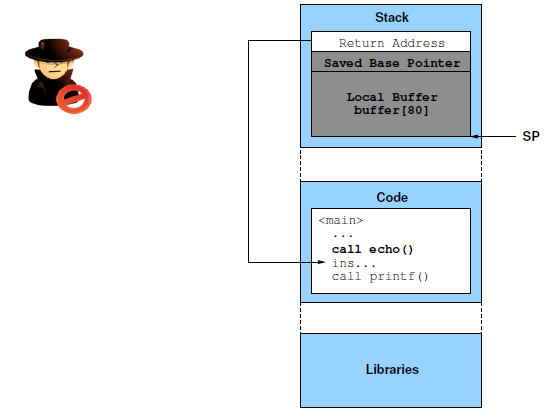
\includegraphics[width=.65\linewidth]{Linux/imagens/bo4.PNG}
    \end{center}

\end{frame}

\begin{frame}{Buffer Overflow}
    \begin{center}
       (6) Invasor insere o código malicioso
       \linebreak
       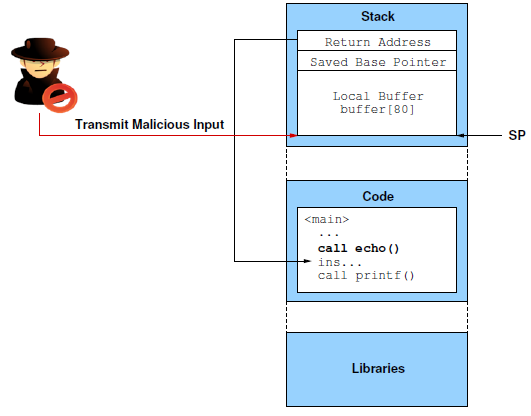
\includegraphics[width=.65\linewidth]{Linux/imagens/bo5.PNG}
    \end{center}

\end{frame}

\begin{frame}{Buffer Overflow}
    \begin{center}
       (7) Código malicioso é um shellcode...
       \linebreak
       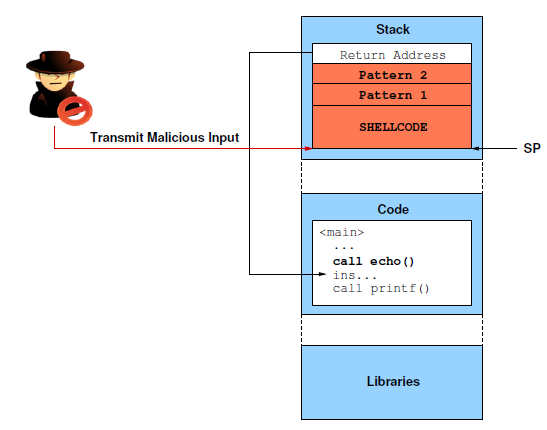
\includegraphics[width=.65\linewidth]{Linux/imagens/bo6.PNG}
    \end{center}

\end{frame}

\begin{frame}{Buffer Overflow}
    \begin{center}
       (8) ... com um novo endereço de retorno
       \linebreak
       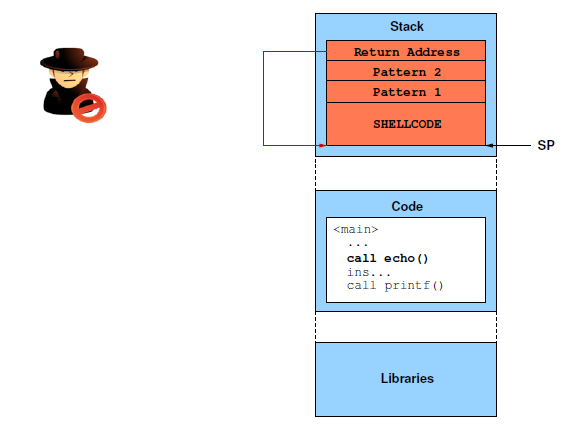
\includegraphics[width=.65\linewidth]{Linux/imagens/bo7.PNG}
    \end{center}

\end{frame}

\begin{frame}{Buffer Overflow}
    \begin{center}
       (9) Antes de echo retornar, SP é atualizado
       \linebreak
       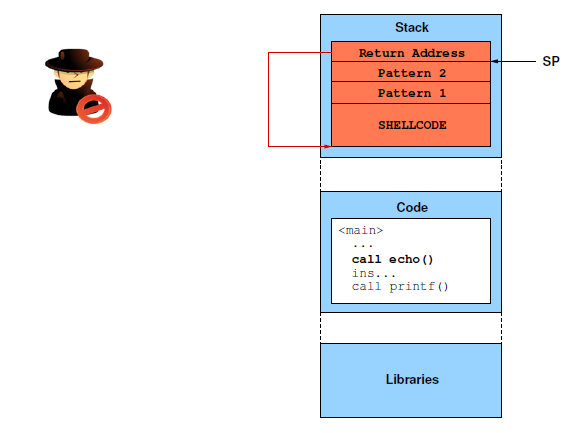
\includegraphics[width=.65\linewidth]{Linux/imagens/bo8.PNG}
    \end{center}

\end{frame}

\begin{frame}{Buffer Overflow}
    \begin{center}
       (10) O endereço de retorno direciona a execução ao shellcode injetado
       \linebreak
       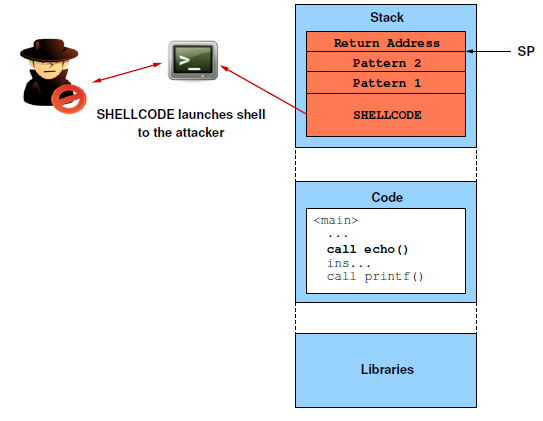
\includegraphics[width=.65\linewidth]{Linux/imagens/bo9.PNG}
    \end{center}

\end{frame}


\begin{frame}{Return to libc}
    \begin{itemize}
        \item {
        Para corrigir a vulnerabilidade buffer overflow, em muitos sistemas UNIX a pilha é não executável
        }
        \item {
        Existem casos em que o buffer é muito pequeno para injeção de código malicioso
        }
        \item{
        return-to-libc não necessita de uma pilha executável (nem usa shellcode)
        }
        \item{
        O princípio básico consiste em fazer a execução pular para um código existente de alguma biblioteca linkada (como libc) - p.e.: a chamada de sistema {\it system()}.
        }
        \item{
        Passando como argumento para essa chamada "/bin/sh" é possível lançar um shell.
            \begin{itemize}
                \item system("/bin/sh")
            \end{itemize}
        }
    \end{itemize}
    
\end{frame}

\begin{frame}{Return to libc}
    \begin{itemize}
        \item {
            Programas que usam funções de uma biblioteca compartilhada como {\it printf} da libc, farão a linkagem da biblioteca como um todo no seu espaço de endereçamento em tempo de execução.
        }
        \item{
            Isso significa que, mesmo que {\it system} nunca seja chamada, seu código (assim como o código de todas as outras funções na libc) é acessível em tempo de execução
        }
    \end{itemize}
    
\end{frame}

\begin{frame}{Return to libc - exemplo}
    \begin{center}
       (1) Invasor transmite entrada maliciosa
       \linebreak
       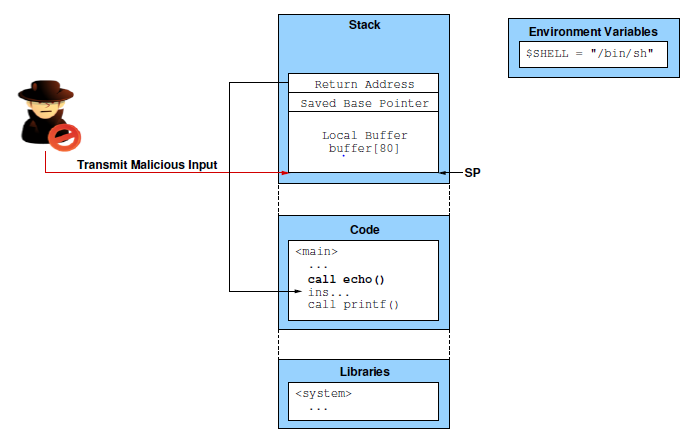
\includegraphics[width=.8\linewidth]{Linux/imagens/rtl1.PNG}
    \end{center}

\end{frame}

\begin{frame}{Return to libc - exemplo}
    \begin{center}
       (2) Pode ser qualquer coisa que ocupe o espaço até o endereço de retorno
       \linebreak
       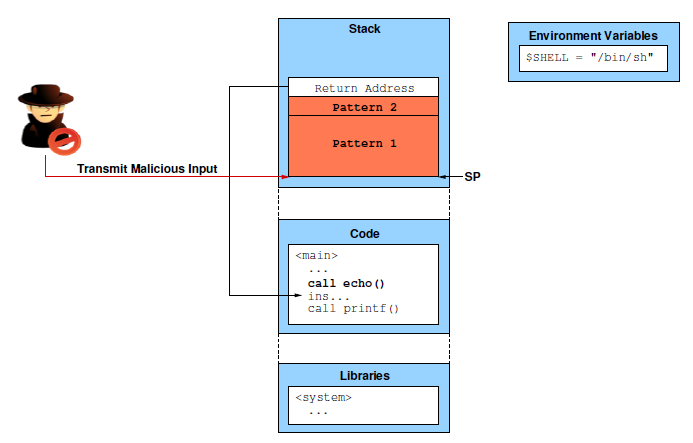
\includegraphics[width=.8\linewidth]{Linux/imagens/rtl2.PNG}
    \end{center}

\end{frame}

\begin{frame}{Return to libc - exemplo}
    \begin{center}
       (3) O endereço de retorno é sobrescrito com o endereço da função system()
       \linebreak
       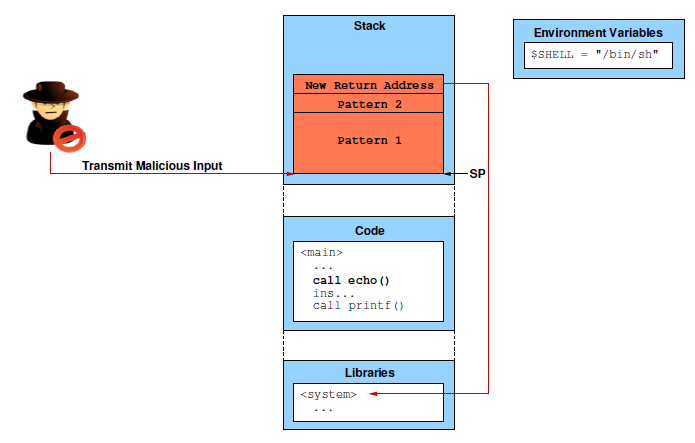
\includegraphics[width=.8\linewidth]{Linux/imagens/rtl3.PNG}
    \end{center}

\end{frame}

\begin{frame}{Return to libc - exemplo}
    \begin{center}
       (4) O endereço de retorno para a função system() é colocado na pilha
       \linebreak
       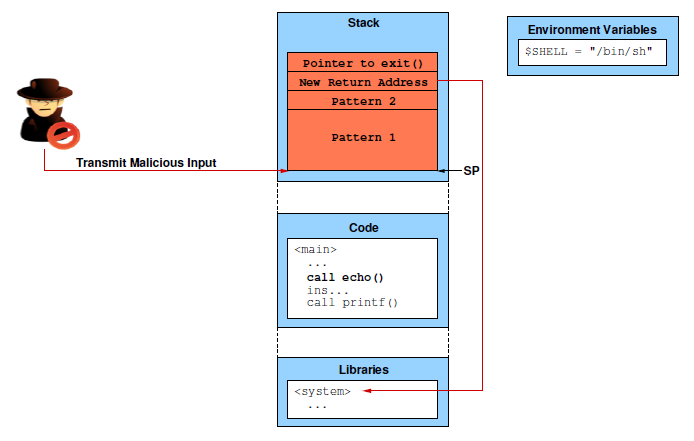
\includegraphics[width=.8\linewidth]{Linux/imagens/rtl4.PNG}
    \end{center}

\end{frame}

\begin{frame}{Return to libc - exemplo}
    \begin{center}
       (5) O endereço da string "/bin/sh" - argumento para system() - é colocado na pilha (p.e.: associando a uma variável ambiente)
       \linebreak
       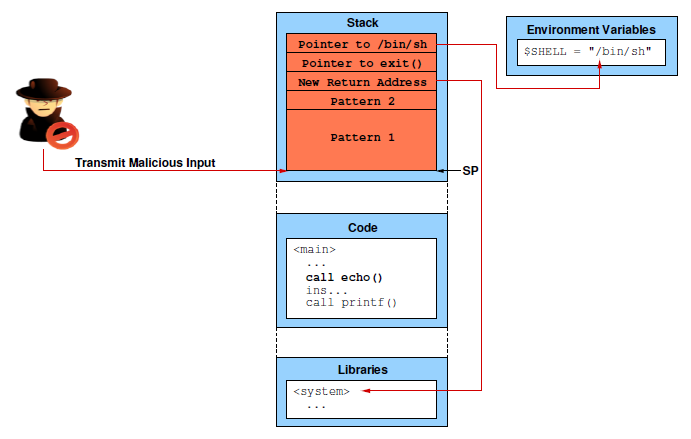
\includegraphics[width=.8\linewidth]{Linux/imagens/rtl5.PNG}
    \end{center}

\end{frame}

\begin{frame}{Return to libc - exemplo}
    \begin{center}
       (6) Quando echo() retorna, um novo shell é lançado
       \linebreak
       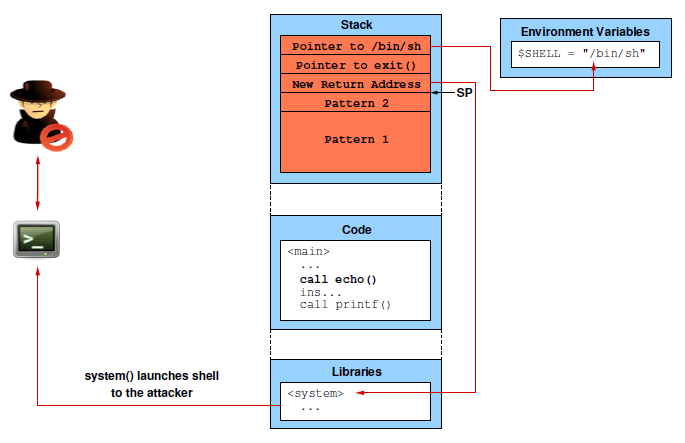
\includegraphics[width=.8\linewidth]{Linux/imagens/rtl6.PNG}
    \end{center}

\end{frame}

\begin{frame}{Return to libc}
  \begin{itemize}
      \item {
      Return to libc consegue superar o mecanismo de defesa Writable Xor Executable
      }
      \item{
      Problemas:
        \begin{itemize}
            \item {
                Invasor necessita das funções da libc
            }
            \item{
                É possível chamar apenas uma função depois da outra, não é possível ramificar as chamadas
            }
        \end{itemize}
      }
  \end{itemize}
\end{frame}

\begin{frame}{Return-Oriented Programming}
    \begin{itemize}
        \item {
            Técnica de ataque que burla o mecanismo de defesa W xor E
        }
        \item{
            Computação Arbitrária (Turing-complete) que não necessita de
            \begin{itemize}
                \item {
                Injeção de Código
                }
                \item{
                chamada para alguma função de alguma bibliteca
                }
                \item{
                modificar o código original
                }
            \end{itemize}
        }
        \item{
         Utiliza uma série de sequência de instruções conhecidas como \textcolor{red}{\bf Gadgets}
        }
        \item{
            A arquitetura x86 não limita as instruções a terem tamanhos específicos
            \begin{itemize}
                \item {
                Isso significa que é possível apontar para o meio de uma instrução válida fazendo com que uma instrução diferente seja executada
                }
            \end{itemize}
        }
    \end{itemize}
    
\end{frame}

\begin{frame}{Return-Oriented Programming}
    \begin{center}
       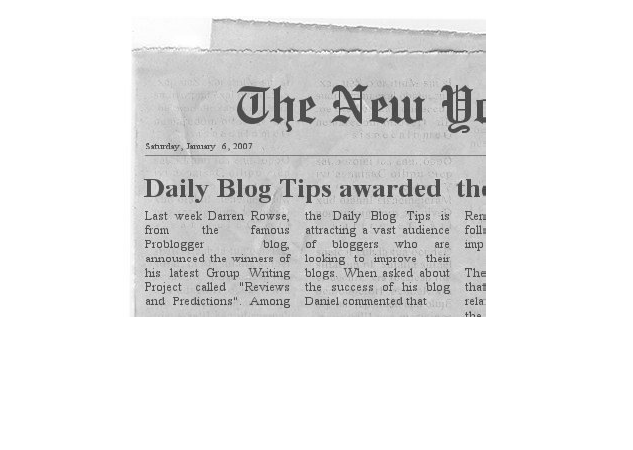
\includegraphics[width=.8\linewidth]{Linux/imagens/j1.PNG}
    \end{center}

\end{frame}

\begin{frame}{Return-Oriented Programming}
    \begin{center}
       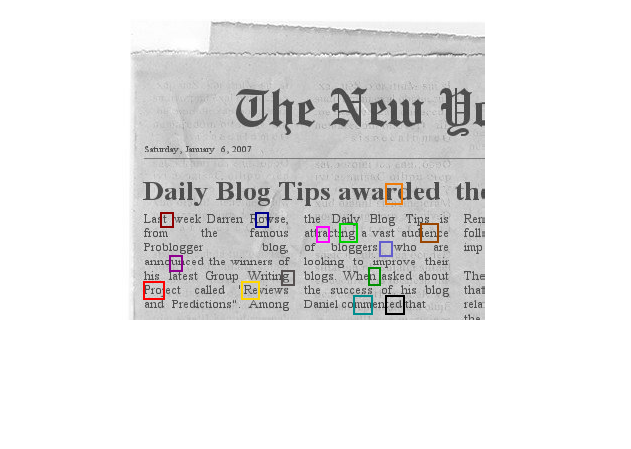
\includegraphics[width=.8\linewidth]{Linux/imagens/j2.PNG}
    \end{center}

\end{frame}

\begin{frame}{Return-Oriented Programming}
    \begin{center}
       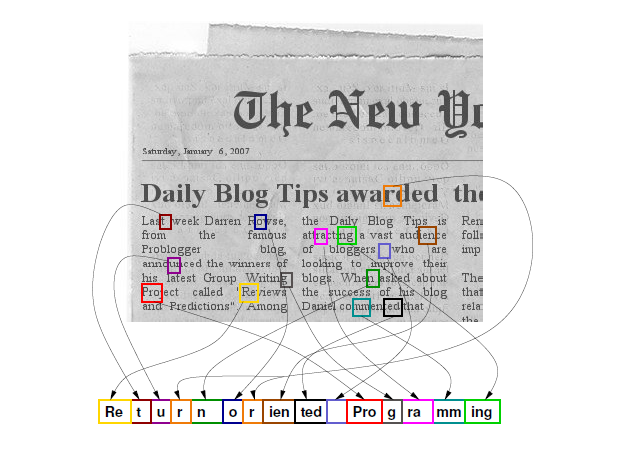
\includegraphics[width=.8\linewidth]{Linux/imagens/j3.PNG}
    \end{center}

\end{frame}

\begin{frame}{Return-Oriented Programming}
    \begin{itemize}
        \item {
        Return-Oriented Programing faz o uso de pequenas sequências de instruções ao invés de utilizar funções inteiras
        }
        \item{
        As sequências de instruções vão de 2 a 5 instruções por sequência
        }
        \item{
        Todas as sequências terminam com uma instrução \textcolor{red}{ret}
        }
        \item{
        As sequências de instruções são encadeadas para formar um Gadget
        }
        \item{
        O gadget vai realizar alguma tarefa específica (p.e.: load, store, ...)
        }
        \item{
        O ataque tem suas ações executadas combinando os gadgets
        }
    \end{itemize}
    
\end{frame}

\begin{frame}{Return-Oriented Programming}
    \begin{center}
       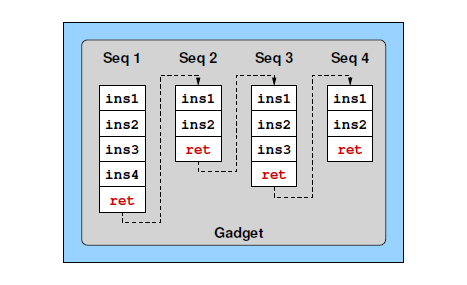
\includegraphics[width=.8\linewidth]{Linux/imagens/gadget.PNG}
    \end{center}

\end{frame}

\begin{frame}{Return-Oriented Programming}
    \begin{center}
       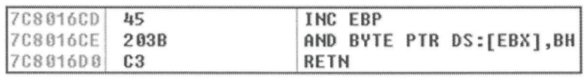
\includegraphics[width=.8\linewidth]{Linux/imagens/gadget1.png}
    \end{center}
    \begin{itemize}
        \item {
            7c8016cc é o endereço da instrução real
        }
        \item {
             Se mudarmos 1 byte, e passarmos a apontar para 7c8016cd, as instruções mudam totalmente:
        }
    \end{itemize}
    
    \begin{center}
       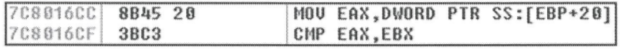
\includegraphics[width=.8\linewidth]{Linux/imagens/gadget2.png}
    \end{center}
    
    \begin{itemize}
        \item {É assim que os gadgets são construídos}
    \end{itemize}

\end{frame}


\begin{frame}{ROP - exemplo}
    \begin{center}
       (1) O programa está esperando a entrada do usuário
       \linebreak
       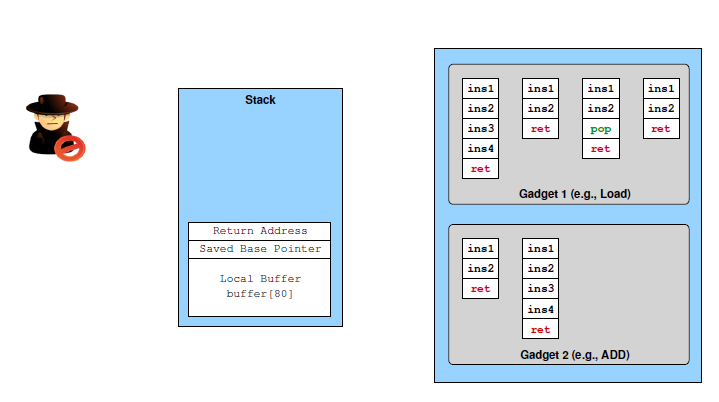
\includegraphics[width=.9\linewidth]{Linux/imagens/rop1.PNG}
    \end{center}

\end{frame}

\begin{frame}{ROP - exemplo}
    \begin{center}
       (2) Buffer Overflow
       \linebreak
       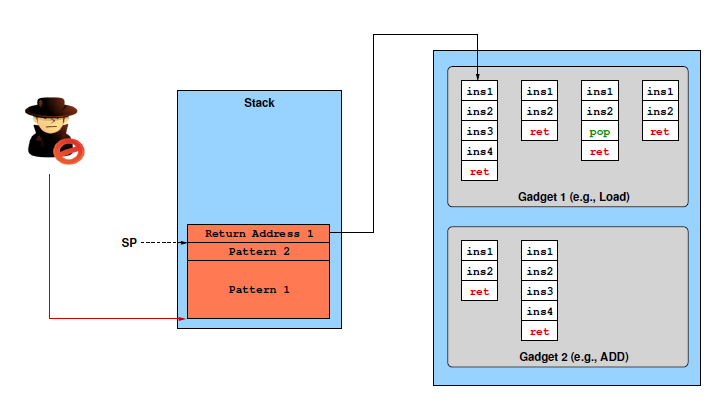
\includegraphics[width=.9\linewidth]{Linux/imagens/rop2.PNG}
    \end{center}

\end{frame}

\begin{frame}{ROP - exemplo}
    \begin{center}
       (3) A entrada contém endereços de retorno e um argumento
       \linebreak
       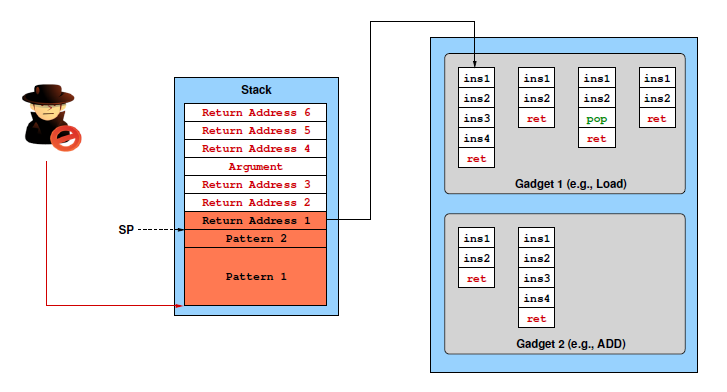
\includegraphics[width=.9\linewidth]{Linux/imagens/rop3.PNG}
    \end{center}

\end{frame}

\begin{frame}{ROP - exemplo}
    \begin{center}
       (4) Com o retorno, a primeira sequência é executada
       \linebreak
       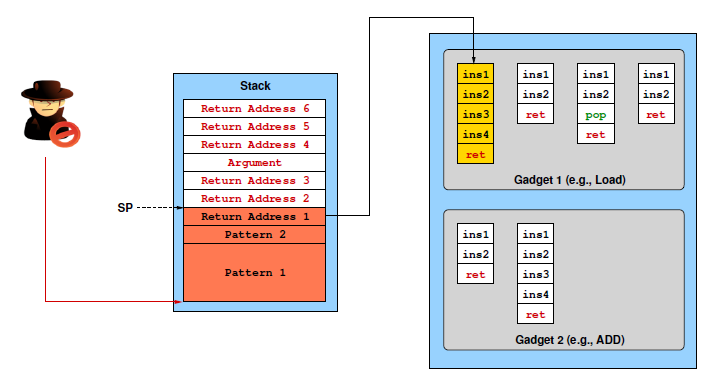
\includegraphics[width=.9\linewidth]{Linux/imagens/rop4.PNG}
    \end{center}

\end{frame}

\begin{frame}{ROP - exemplo}
    \begin{center}
       (5) A instrução de retorno transfere o controle para a próxima sequência de instruções
       \linebreak
       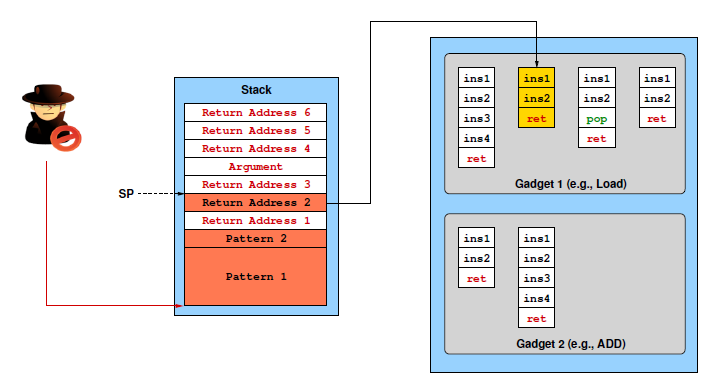
\includegraphics[width=.9\linewidth]{Linux/imagens/rop5.PNG}
    \end{center}

\end{frame}

\begin{frame}{ROP - exemplo}
    \begin{center}
       (6) Retorno da sequência 2 transfere controle para sequência 3
       \linebreak
       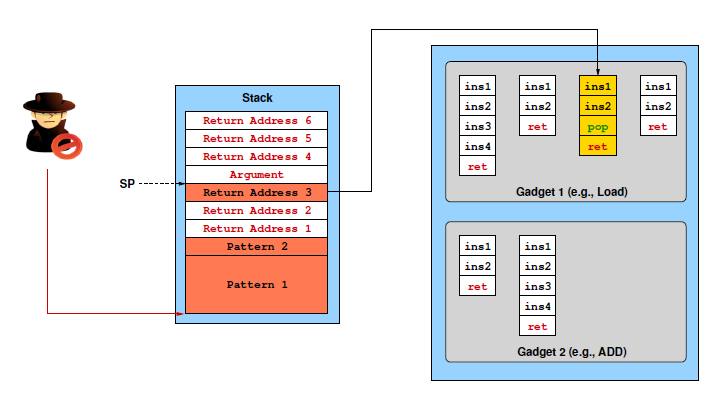
\includegraphics[width=.9\linewidth]{Linux/imagens/rop6.PNG}
    \end{center}

\end{frame}

\begin{frame}{ROP - exemplo}
    \begin{center}
       (7) Pop do argumento da Pilha
       \linebreak
       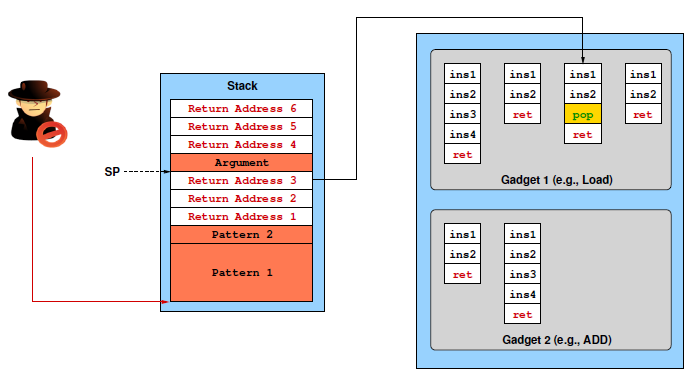
\includegraphics[width=.9\linewidth]{Linux/imagens/rop7.PNG}
    \end{center}

\end{frame}

\begin{frame}{ROP - exemplo}
    \begin{center}
       (8) Retorno da sequência de instruções 3
       \linebreak
       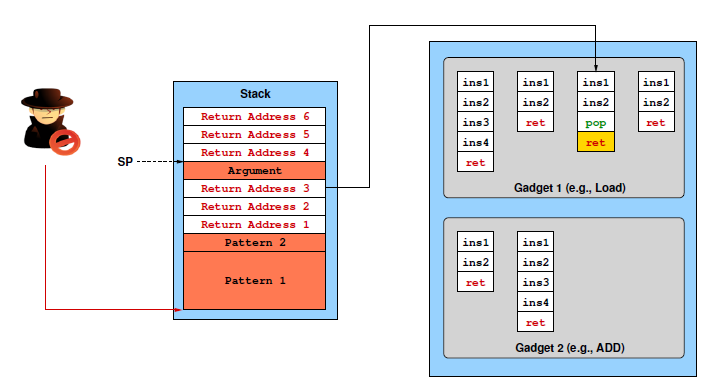
\includegraphics[width=.9\linewidth]{Linux/imagens/rop8.PNG}
    \end{center}

\end{frame}


\begin{frame}{ROP - exemplo}
    \begin{center}
       (9) Retorno passa o fluxo de execução para a sequência 4
       \linebreak
       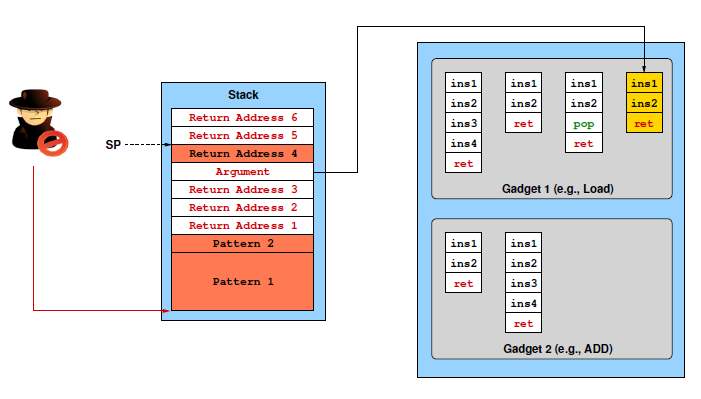
\includegraphics[width=.9\linewidth]{Linux/imagens/rop9.PNG}
    \end{center}

\end{frame}

\begin{frame}{ROP - exemplo}
    \begin{center}
       (10) Retorno da sequência 4 transfere o controle pro segundo gadget
       \linebreak
       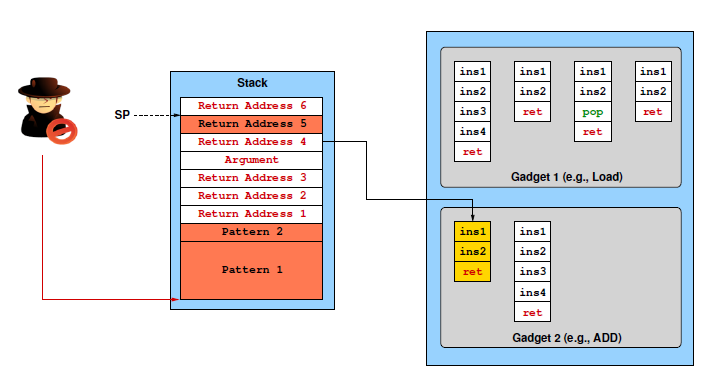
\includegraphics[width=.9\linewidth]{Linux/imagens/rop10.PNG}
    \end{center}

\end{frame}

\begin{frame}{ROP - exemplo}
    \begin{center}
       (11) Retorno da sequência 1 transfere controle para sequência 2
       \linebreak
       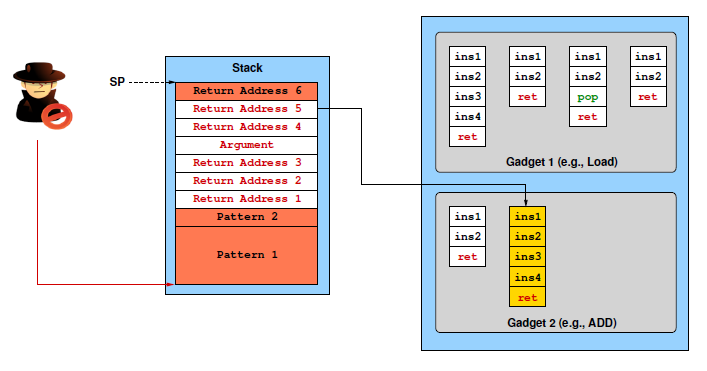
\includegraphics[width=.9\linewidth]{Linux/imagens/rop11.PNG}
    \end{center}

\end{frame}



\begin{frame}{Stack Pivoting}

    \begin{itemize}
        \item {
        Método que move a posição de ESP da pilha para alguma área como a heap
        }
    \end{itemize}
    \begin{center}
    {\bf xchg/mov esp, eax} \linebreak
    {\bf ret}
    \end{center}
    \begin{itemize}
        \item {
            Funciona lado a lado com ROP
        }
    \end{itemize}
    
\end{frame}


% You can reveal the parts of a slide one at a time
% with the \pause command:
\begin{frame}{Second Slide Title}
  \begin{itemize}
  \item {
    First item.
    \pause % The slide will pause after showing the first item
  }
  \item {   
    Second item.
  }
  % You can also specify when the content should appear
  % by using <n->:
  \item<3-> {
    Third item.
  }
  \item<4-> {
    Fourth item.
  }
  % or you can use the \uncover command to reveal general
  % content (not just \items):
  \item<5-> {
    Fifth item. \uncover<6->{Extra text in the fifth item.}
  }
  \end{itemize}
\end{frame}

\section{Exploiting Windows for PenTesters}
\subsection{Mecanismos de Defesa}

\begin{frame}{Write xor Execute e DEP}

  \begin{itemize}
  \item{
  O que faz:
  \begin{itemize}
    \item{
    Se baseia em marcar segmentos de memória que apenas seria possível alterar (write) ou apenas executar (execute). O DEP (Data Execution Prevention) é baseado no Write xor Execute do Linux, tem principio de que nenhum código de execução seja na pilha ou monte. Qualquer tentativa de execução de um código marcado como não executável não será executado.

    }
  \end{itemize}
  }
  \item{
  Como explorar:
  \begin{itemize}
      \item {
      Caso seja uma parte apenas executável e o código a ser executado já esteja dentro da aplicação, só é preciso retornar e executar a parte do código desejada. Caso seja uma parte que apenas tenha permissão para modificar é possível retornar para a parte desejada utilizando  um shellcode. Dependendo do OS é possível desativar esse mecanismo.
      }
  \end{itemize}      
    }
\end{itemize}
\end{frame}

\begin{frame}{Flag SafeSEH}

  \begin{itemize}
  \item{
  O que faz:
  \begin{itemize}
    \item{
    É uma flag que quando utilizada, o linker do projeto faz uma tabela de operadores válidos e caso o programa sobrescreva o operador e seu endereço não estiver na tabela como um operador válido o programa é terminado.
    }
  \end{itemize}
  }
  \item{
  Como explorar:
  \begin{itemize}
      \item {
       Seu maior problema é que muitos programas feito por terceiros não são feitos utilizando a flag SafeSEH (Safe Structured Exception Handling) o que da chance à ataques nas áreas de memória não protegidas.
      }
  \end{itemize}      
    }
\end{itemize}
\end{frame}


\begin{frame}{PEB Randomization}

  \begin{itemize}
  \item{
  O que faz:
  \begin{itemize}
    \item{
    Utiliza vários endereços (16 em total, de 0x7FFD000 até 0x7FFDF000) para o Process Environment Block em cada execução do programa.
    }
  \end{itemize}
  }
  \item{
  Como explorar:
  \begin{itemize}
      \item {
      É possível sobrescrever RtlCriticalSection para que ele sobrescreva a saída do programa, dentre outros tipos de ataque.  Pesquisa da Symantec mostrou que é possível ter acerto de 25\% na primeira tentativa na localização do PEB. Como existem um número limitado de endereços, caso seja possível inúmeras tentativas de achar o endereço o sucesso de ataque é iminente.

      }
      \end{itemize}  
    }
      
\end{itemize}
\end{frame}

\begin{frame}{Heap Cookies}

  \begin{itemize}
  \item{
  O que faz:
  \begin{itemize}
    \item{
    Tem comprimento de 8 bits e fornece 256 chaves diferentes usadas para proteger um bloco de memória.
    }
  \end{itemize}
  }
  \item{
  Como explorar:
  \begin{itemize}
      \item {
       Parecido com PEB randomization, como existem possibilidades finitas, a média de sucesso na tentativa de ter a chave certa é de 1/256. Portando é possível burlar essa defesa com força bruta ou memory leaks.

      }
       \end{itemize}
    }

\end{itemize}
\end{frame}

\begin{frame}{Visual C++/GS Check}

  \begin{itemize}
  \item{
  O que faz:
  \begin{itemize}
    \item{
    Força um cookie de segurança de 32 bits na pilha de execução se for determinado que o programa é vulnerável, assim protegendo o endereço de retorno, para cada módulo carregado é feito um cookie. No retorno de funções é feito a checagem do cookie, em caso de falha o processo é interrompido.
    }
  \end{itemize}
  }
  \item{
  Como explorar:
  \begin{itemize}
      \item {
      Qualquer programa que foi compilado sem utilizar o MS Visual Studio precisará ser recompilado para incluir essa proteção, portanto nem todos os programas possuirão essa proteção.

      }
  \end{itemize}      
    }
      
\end{itemize}
\end{frame}

\begin{frame}{Safe Unlinking}

\begin{itemize}
  \item{
  O que faz:
  \begin{itemize}
    \item{
    De maneira similar ao unlink() utilizado no Linux, os ponteiros do programa são testados de modo que para onde eles apontem ainda apontem para si antes de haver o unlink, ((B->Flink)->Blink B \&\& (B->Blink)->Flink B), ou seja, o ponteiro de volta da próxima parte deve estar apontando para a parte atual do código e o ponteiro de ida da parte anterior do código deve estar apontando também para a parte atual.
    }
  \end{itemize}
  }
\end{itemize}
\end{frame}

\begin{frame}{LFH (Low Fragmentation Heap)}

  \begin{itemize}
  \item{
  O que faz:
  \begin{itemize}
    \item{
    É colocado um cookie de 32 bits no início para garantir a integridade via checagem quando são alocados blocos de buckets. LHF pode alocar blocos maiores que 8 bits mas menores que 16 bits, alocações maiores que 16 bits é utilizado o heap padrão e o cookie de 32 bits não será utilizado.
    }
  \end{itemize}
  }
\end{itemize}
\end{frame}

\begin{frame}{ASLR (Adress Space Layout Randomization)}

  \begin{itemize}
  \item{
  O que faz:
  \begin{itemize}
    \item{
    Durante a inicialização um módulo que utiliza ASLR, é escolhido um de 256 endereços possíveis, o endereço que foi carregado permanece até a reinicialização do sistema. Incluindo a randomização do executável, também é randomizado a pilha, heap e as bibliotecas utilizadas. \linebreak(Obs.: PEB randomization é feito em um processo separado)
    }
  \end{itemize}
  }
  \item{
  Como explorar:
  \begin{itemize}
      \item {
      Como já visto é necessário acertar o endereço que foi utilizado, então no caso de várias tentativas o êxito é propínquo. Muitos computadores não utilizam Windows VISTA em diante e não possuem o ALSR nativo.

      }
      \end{itemize}
    }

\end{itemize}
\end{frame}

% Placing a * after \section means it will not show in the
% outline or table of contents.
\section*{Summary}

\begin{frame}{Summary}
  \begin{itemize}
  \item
    Mecanismos de defesa do Windows.
  \item
    Linking e Loading no Windows.
  \item
    Ferramentas a serem utilizadas.
  \end{itemize}
  
  \begin{itemize}
  \item
    Outlook
    \begin{itemize}
    \item
      Something you haven't solved.
    \item
      Something else you haven't solved.
    \end{itemize}
  \end{itemize}
\end{frame}



% All of the following is optional and typically not needed. 
\appendix
\section<presentation>*{\appendixname}
\subsection<presentation>*{For Further Reading}

\begin{frame}[allowframebreaks]
  \frametitle<presentation>{For Further Reading}
    
  \begin{thebibliography}{10}
    
  \beamertemplatebookbibitems
  % Start with overview books.

  \bibitem{Author1990}
    A.~Author.
    \newblock {\em Handbook of Everything}.
    \newblock Some Press, 1990.
 
    
  \beamertemplatearticlebibitems
  % Followed by interesting articles. Keep the list short. 

  \bibitem{Someone2000}
    S.~Someone.
    \newblock On this and that.
    \newblock {\em Journal of This and That}, 2(1):50--100,
    2000.
  \end{thebibliography}
\end{frame}

\end{document}



